\begin{figure}
  \centering 
  \begin{subfigure}[b]{0.45\textwidth}
    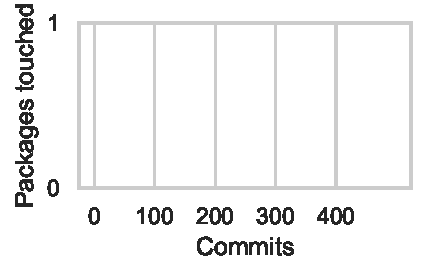
\includegraphics[width=\textwidth]{sections/results/packages/time_series_components_touched.packages.sustained.founder.commits_500.pdf}
    \caption{Sustained founder (n=27, $\mu$=35.85, median=15.0 \& std=29.7)}
    \label{subfig:sections/results/packages/time_series_components_touched_packages_sustained_founder_commits_500_pdf}
  \end{subfigure}
  \begin{subfigure}[b]{0.45\textwidth}
    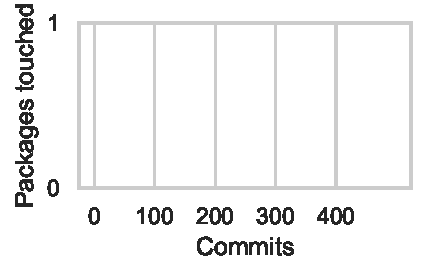
\includegraphics[width=\textwidth]{sections/results/packages/time_series_components_touched.packages.sustained.later.joiner.commits_500.pdf}
    \caption{Sustained later joiner (n=203, $\mu$=37.08, median=22.0 \& std=36.82)}
    \label{subfig:sections/results/packages/time_series_components_touched_packages_sustained_later_joiner_commits_500_pdf}
  \end{subfigure}
\caption[Time Series for packages unit:commits category:2 commits:all]{A time series for the all commits, excluding transient, with the average mean (blue line), packages touched (y-axis) against the number of commits (x-axis) for two (2) developer categories. Green is the standard deviation above the mean, and pink is the standard deviation below the mean.} 
    \label{fig:codebase_graph_latex_repository_graph_component_time_series_time_series_components_touchedpackages_0_500}
\end{figure}
\clearpage 
\begin{figure}
  \centering 
  \begin{subfigure}[b]{0.45\textwidth}
    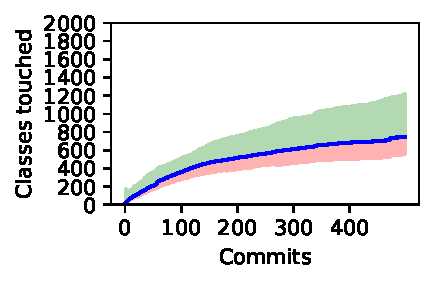
\includegraphics[width=\textwidth]{sections/results/classes/time_series_components_touched.classes.sustained.founder.commits_500.pdf}
    \caption{Sustained founder (n=27, $\mu$=833.11, median=482.0 \& std=428.64)}
    \label{subfig:sections/results/classes/time_series_components_touched_classes_sustained_founder_commits_500_pdf}
  \end{subfigure}
  \begin{subfigure}[b]{0.45\textwidth}
    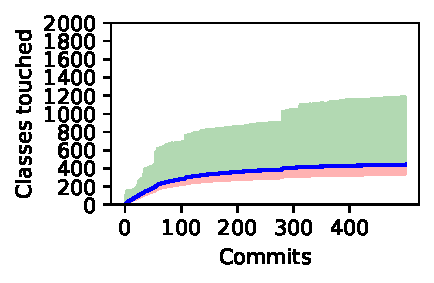
\includegraphics[width=\textwidth]{sections/results/classes/time_series_components_touched.classes.sustained.later.joiner.commits_500.pdf}
    \caption{Sustained later joiner (n=203, $\mu$=442.33, median=239.0 \& std=426.23)}
    \label{subfig:sections/results/classes/time_series_components_touched_classes_sustained_later_joiner_commits_500_pdf}
  \end{subfigure}
\caption[Time Series for classes unit:commits category:2 commits:all]{A time series for the all commits, excluding transient, with the average mean (blue line), classes touched (y-axis) against the number of commits (x-axis) for two (2) developer categories. Green is the standard deviation above the mean, and pink is the standard deviation below the mean.} 
    \label{fig:codebase_graph_latex_repository_graph_component_time_series_time_series_components_touchedclasses_0_500}
\end{figure}
\clearpage 
\begin{figure}
  \centering 
  \begin{subfigure}[b]{0.45\textwidth}
    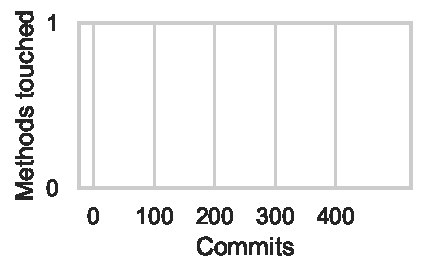
\includegraphics[width=\textwidth]{sections/results/methods/time_series_components_touched.methods.sustained.founder.commits_500.pdf}
    \caption{Sustained founder (n=27, $\mu$=3477.96, median=1727.0 \& std=2190.78)}
    \label{subfig:sections/results/methods/time_series_components_touched_methods_sustained_founder_commits_500_pdf}
  \end{subfigure}
  \begin{subfigure}[b]{0.45\textwidth}
    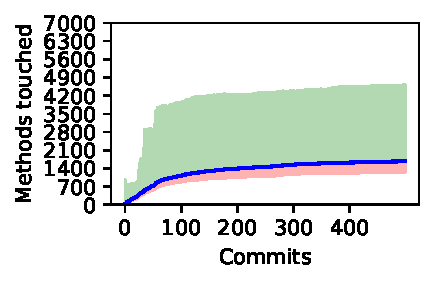
\includegraphics[width=\textwidth]{sections/results/methods/time_series_components_touched.methods.sustained.later.joiner.commits_500.pdf}
    \caption{Sustained later joiner (n=203, $\mu$=1672.84, median=838.0 \& std=1909.9)}
    \label{subfig:sections/results/methods/time_series_components_touched_methods_sustained_later_joiner_commits_500_pdf}
  \end{subfigure}
\caption[Time Series for methods unit:commits category:2 commits:all]{A time series for the all commits, excluding transient, with the average mean (blue line), methods touched (y-axis) against the number of commits (x-axis) for two (2) developer categories. Green is the standard deviation above the mean, and pink is the standard deviation below the mean.} 
    \label{fig:codebase_graph_latex_repository_graph_component_time_series_time_series_components_touchedmethods_0_500}
\end{figure}
\clearpage 
